\section{SSSP}
\subsection{Dijkstra}
\begin{frame}
\frametitle{Das Problem}
\begin{block}{Das Problem}
SSSP schlägt bei gewichteten Graphen fehl: 

\begin{figure}
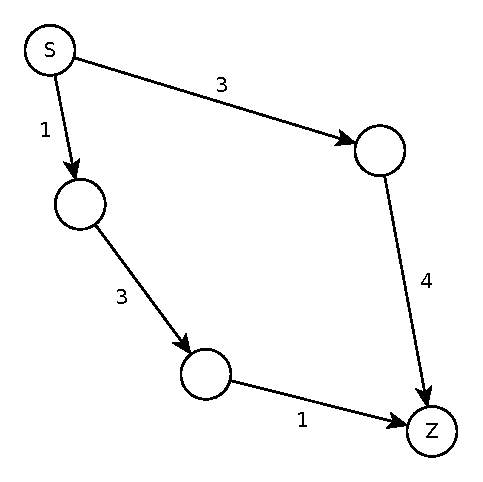
\includegraphics[scale=.75]{dijkstra_graphs/bfs_fail_0.pdf}
\end{figure}

\end{block}
\end{frame}

\begin{frame}
\frametitle{Das Problem}
\begin{figure}
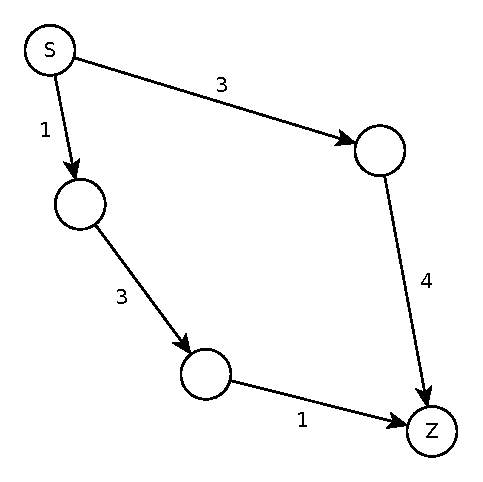
\includegraphics[scale=.8]{dijkstra_graphs/bfs_fail_0.pdf}
\end{figure}
\end{frame}

\begin{frame}
\frametitle{Das Problem}
\begin{figure}
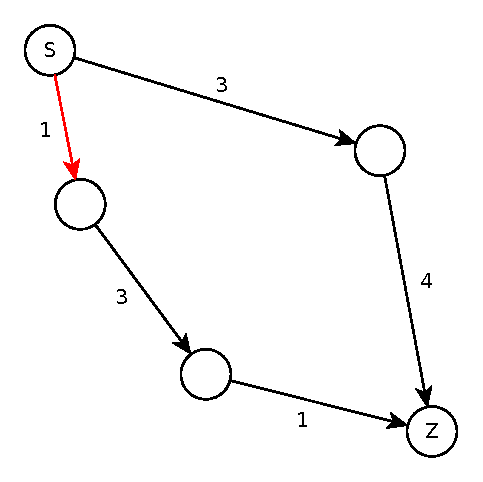
\includegraphics[scale=.8]{dijkstra_graphs/bfs_fail_1.pdf}
\end{figure}
\end{frame}

\begin{frame}
\frametitle{Das Problem}
\begin{figure}
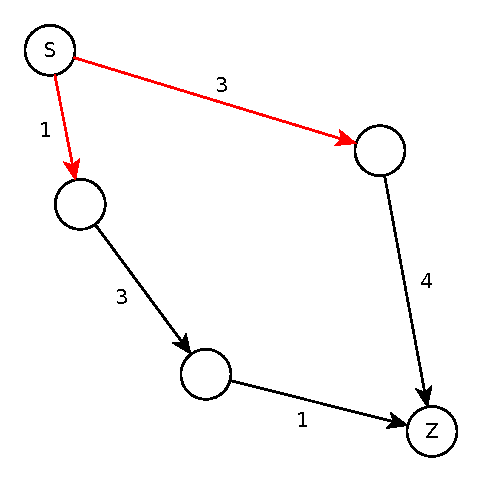
\includegraphics[scale=.8]{dijkstra_graphs/bfs_fail_2.pdf}
\end{figure}
\end{frame}

\begin{frame}
\frametitle{Das Problem}
\begin{figure}
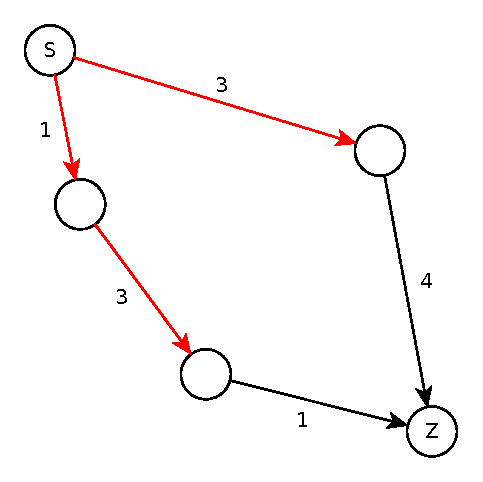
\includegraphics[scale=.8]{dijkstra_graphs/bfs_fail_3.pdf}
\end{figure}
\end{frame}

\begin{frame}
\frametitle{Das Problem}
\begin{figure}
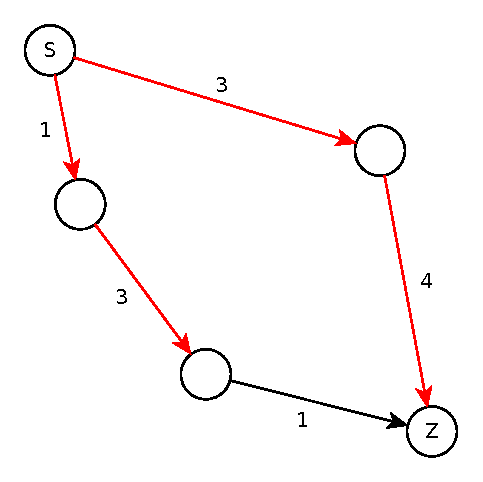
\includegraphics[scale=.8]{dijkstra_graphs/bfs_fail_4.pdf}
\end{figure}
\end{frame}

\begin{frame}
\frametitle{Das Problem}
\begin{figure}
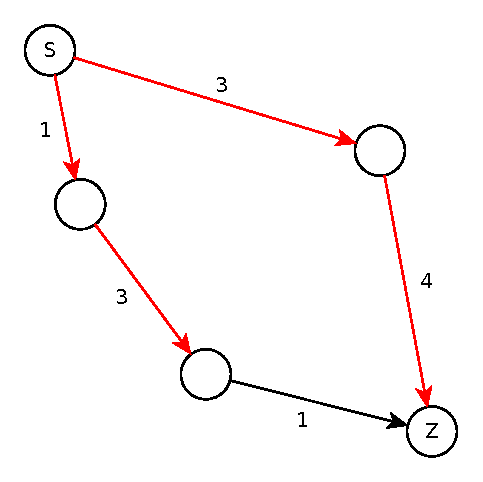
\includegraphics[scale=.8]{dijkstra_graphs/bfs_fail_4.pdf}
\end{figure}

$\implies$ Es wird ein Weg der Länge $7$ gefunden, obwohl $5$ das Optimum ist

\end{frame}

